\documentclass[10pt,a4paper]{article}
\usepackage[utf8]{inputenc}
\usepackage[T1]{fontenc,url}
\usepackage{multicol}
\usepackage{multirow}
\usepackage{parskip}
\usepackage{lmodern}
\usepackage{microtype}
\usepackage{verbatim}
\usepackage{amsmath, amssymb}
\usepackage{tikz}
\usepackage{physics}
\usepackage{mathtools}
\usepackage{algorithm}
\usepackage{algpseudocode}
\usepackage{listings}
\usepackage{enumerate}
\usepackage{enumitem}
\usepackage{graphicx}
\usepackage{float}
\usepackage{hyperref}
\usepackage{tabularx}
\usepackage{siunitx}
\usepackage{fancyvrb}
\usepackage{minted}
\usepackage{xcolor}
\usepackage{pdfpages}
\usepackage[margin=2cm]{geometry}
\renewcommand{\baselinestretch}{1}
\renewcommand{\b}{\textbf}
\renewcommand{\exp}{e^}

\usemintedstyle{pastie}

\begin{document}

\title{STK1100 -- Oblig 1}
\author{
    \begin{tabular}{r l}
        Jonas Gahr Sturtzel Lunde & (\texttt{jonassl})
    \end{tabular}}
\date{}    % if commented out, the date is set to the current date

\maketitle


Kode og figurer ligger til slutt.

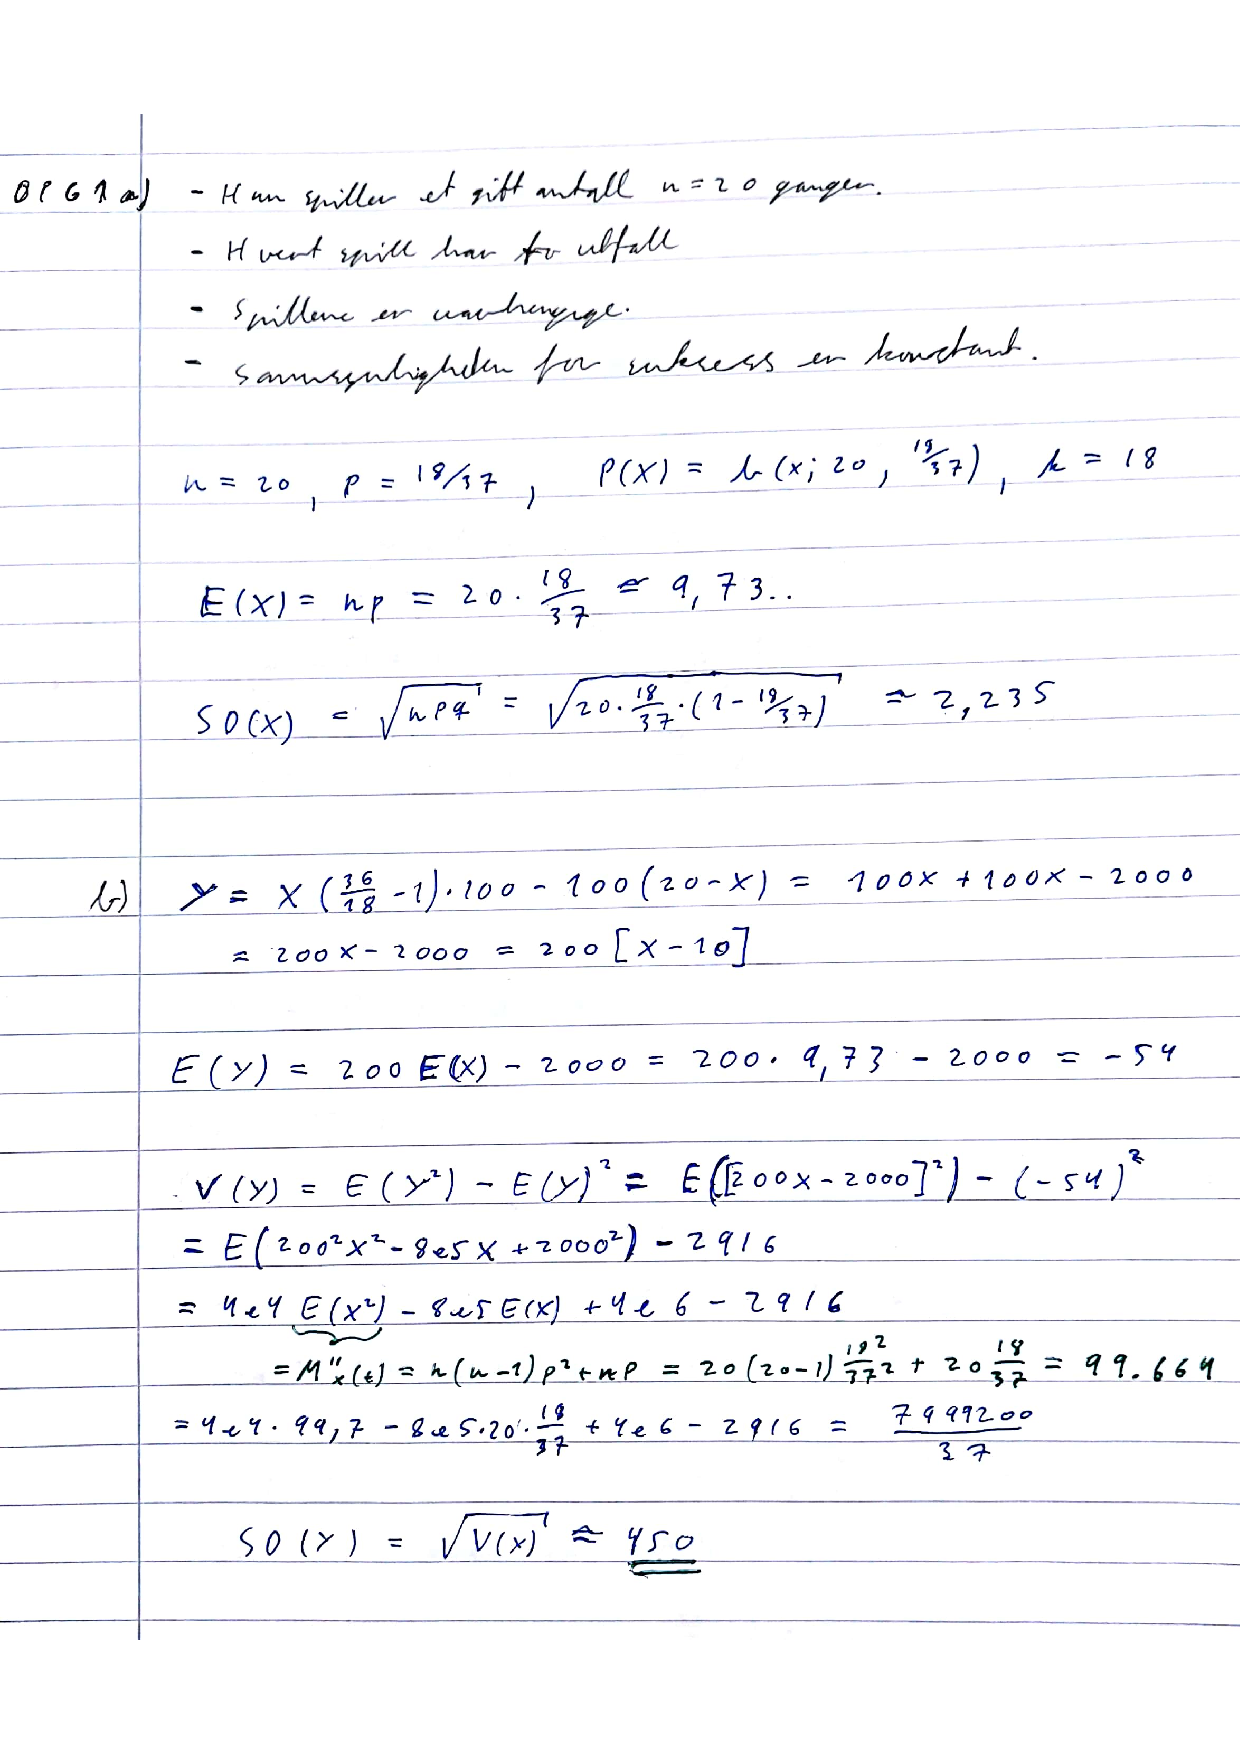
\includepdf[pages={1-}, scale=0.8]{text.pdf}


\section*{Oppgave 1c and 1d}
\inputminted[frame=single, fontsize=\footnotesize]{Python}{src/1cd.py}


\section*{Oppgave 1e og f}
\inputminted[frame=single, fontsize=\footnotesize]{Python}{src/1ef.py}


\section*{Oppgave 2c}
\inputminted[frame=single, fontsize=\footnotesize]{Python}{src/2c.py}
\begin{figure}[H]
\centering
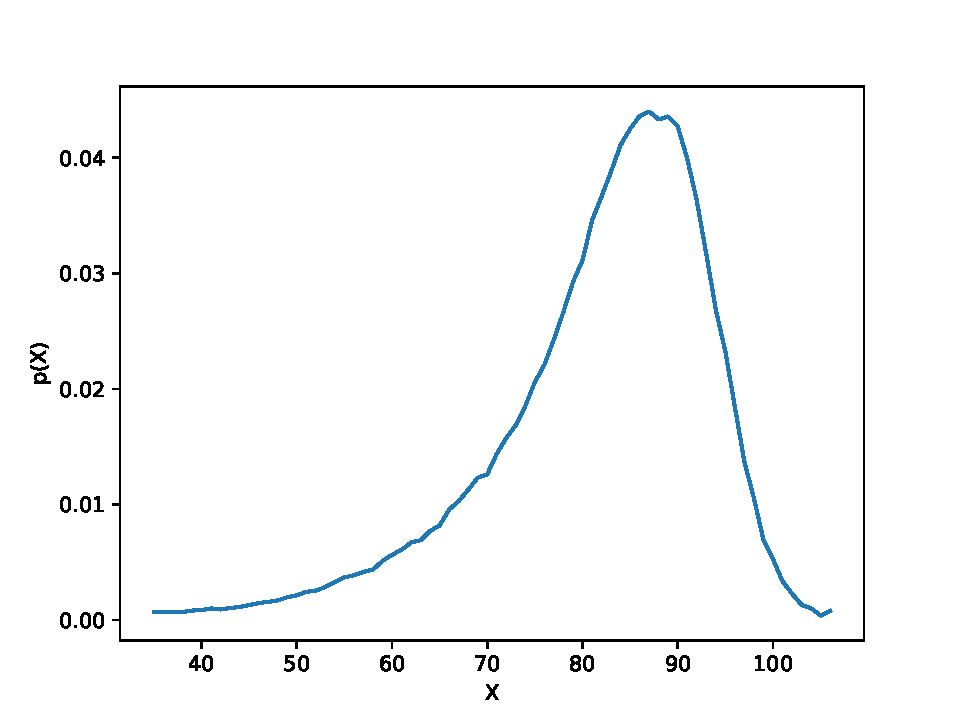
\includegraphics[width=0.6\textwidth]{2c.pdf}
\end{figure}


\section*{Oppgave 2f}
\inputminted[frame=single, fontsize=\footnotesize]{Python}{src/2f.py}


\section*{Oppgave 2i}
\inputminted[frame=single, fontsize=\footnotesize]{Python}{src/2i.py}


\end{document}